\documentclass[11pt]{article}
\usepackage[margin=1in]{geometry}
\usepackage{amsmath,amssymb}
\usepackage{booktabs}
\usepackage{longtable}
\usepackage{enumitem}
\usepackage{graphicx}
\usepackage[hidelinks]{hyperref}
% \fred{CODE} hyperlinks a FRED series code to its series page.
\newcommand{\fred}[1]{\href{https://fred.stlouisfed.org/series/#1}{\texttt{#1}}}

\title{Reproducing ``Mapping Heat in the U.S.\ Financial System''\\ from Public Data}
\author{A self-contained replication guide}
\date{October 2026}

\begin{document}
\maketitle

\begin{abstract}
The Federal Reserve FEDS Notes \textit{Mapping Heat in the U.S.\ Financial
System} (August 2015) builds a heat map of financial-system vulnerabilities
from 44 indicators grouped into 14 components.  This paper documents a full
replication of that exercise from public data alone.  Every indicator is
rebuilt from a named public source with its exact construction given; the
index pipeline is specified formula by formula; and the results are scored
against the paper's own published ``accessible materials'' tables.
43 of 44 indicators are replicated with public proxies (transformed-signal
correlations 0.37--1.00, median 0.91); the documented pipeline
reproduces the published component indices at correlations 0.85--0.98 for
13 of 14 components (aggregate 0.97), and the end-to-end public-proxy panel
tracks the published aggregate index at 0.93.  Two orientation corrections
to the paper's data appendix were required, both discovered empirically.
The one indicator with no workable public proxy (the weighted-average
maturity gap at commercial banks) and the one component the documented
pipeline cannot reproduce even on the paper's own data (commercial real
estate) are documented as findings.  A reader with only this document and
internet access can reproduce the entire exercise.
\end{abstract}

\tableofcontents
\newpage

\section{The original paper}
\label{sec:original}

The Federal Reserve FEDS Notes \textit{Mapping Heat in the U.S.\ Financial
System} (August 2015;
\url{https://www.federalreserve.gov/econres/feds/mapping-heat-in-the-us-financial-system.htm};
data through 2015Q1, sample 1990Q1--2014Q4) proposes
a framework for assessing the build-up of vulnerabilities in the U.S.\
financial system.  It collects \textbf{44 indicators} of financial and
balance-sheet conditions, groups them into \textbf{14 components}
spanning three broad vulnerability categories---valuation pressures,
nonfinancial-sector borrowing, and financial-sector health---and develops
an algorithmic monitoring approach meant to complement the judgmental
assessments typical of official-sector bodies.

The visualization is a \textbf{heat map}: each indicator and each component
is rendered as a color from blue (subdued) to red (acute), where every
cell is the indicator's quantile in its own historical distribution.
Colors are relative to history, not absolute levels.  The paper's headline
empirical claims: the summary vulnerability measures pick up rising
imbalances through the mid-2000s, presaging the financial crisis, and they
lead the credit-to-GDP gap (a key Basel~III gauge) by a year or more,
making them potentially useful for setting macroprudential tools such as
the countercyclical capital buffer.

The 14 components and their indicators are:

\begin{enumerate}[nosep]
\item \textbf{Equity markets:} E/P minus 10-year Treasury yield; E/P ratio.
\item \textbf{Price volatility:} VIX; CDS premium.
\item \textbf{Business credit:} BBB spread; high-yield spread; junk plus
leveraged-loan issuance; C\&I lending standards.
\item \textbf{Commercial real estate:} CRE prices; change in CRE lending
standards.
\item \textbf{Residential real estate:} FICO scores; house prices relative
to rents; change in mortgage lending standards.
\item \textbf{Nonfinancial business:} real debt growth; net leverage of
risky firms; deep-junk issuance share; interest expenses; debt-to-income
ratio.
\item \textbf{Consumer credit:} consumer credit/GDP; consumer debt service
ratio; riskier-borrower debt/DPI; rapid-borrowing incidence.
\item \textbf{Home mortgages:} mortgage debt/GDP; mortgage debt service
ratio; riskier-borrower mortgage debt/DPI; piggy-back incidence;
rapid-borrowing incidence.
\item \textbf{Net saving:} household saving/GDP; nonfinancial business
saving/GDP.
\item \textbf{Bank leverage:} tangible common equity/assets; Tier~1 common
equity ratio; total capital ratio.
\item \textbf{Nonbank leverage:} broker-dealer financing; broker-dealer
leverage ratio; non-agency securitization/GDP.
\item \textbf{Maturity transformation:} loans/deposits; weighted-average
maturity gap; net short-term wholesale debt/GDP.
\item \textbf{Short-term wholesale funding:} gross short-term wholesale
debt/GDP; short-term money share of BHC assets; runnable money-like
liabilities/GDP.
\item \textbf{Size/concentration:} financial-sector liabilities/GDP; top-5
BHC asset share; illiquidity concentration.
\end{enumerate}

\section{The index construction}
\label{sec:pipeline}

Every indicator passes through an identical pipeline.  Let $x_{i,t}$ be the
raw quarterly series for indicator $i$, $t$ indexing quarters.  The
estimation sample is 1990Q1--2014Q4 (100 quarters); series with shorter
histories use their full available span at every step.

\paragraph{Step 1 -- sign orientation.}
Each series is multiplied by $s_i \in \{+1,-1\}$ so that higher values mean
greater vulnerability:
\begin{equation}
y_{i,t} = s_i \cdot T(x_{i,t}).
\end{equation}
Spreads and volatility enter with $s_i=-1$ on their logged values:
compressed spreads and low volatility read as \textit{complacency}, which
the paper treats as the vulnerable state.  Capital ratios enter with
$-1$ (higher capital = safer); saving rates with $-1$ (higher saving =
less vulnerable); lending standards with $-1$ (net tightening = safer).
The exact sign per indicator is listed in Table~\ref{tab:spec}.

\paragraph{Step 2 -- transform $T$.}
One of three transforms:
\begin{itemize}[nosep]
\item \texttt{log}: $T(x_t)=\ln x_t$ (natural log; strictly positive,
right-skewed series: VIX, CDS premium, BBB and high-yield spreads,
junk/leveraged-loan issuance);
\item \texttt{ma10}: $T(x_t)=x_t - \bar{x}_{t}^{(40)}$, where
$\bar{x}_{t}^{(40)}$ is the trailing 40-quarter moving average computed
with a minimum of 20 observations (the first up to 19 quarters are
missing).  Used for ratio-to-GDP series and other trending levels, so the
index responds to the \textit{cyclical} component;
\item \texttt{none}: $T(x_t)=x_t$.
\end{itemize}

\paragraph{Step 3 -- standardize.}
\begin{equation}
z_{i,t} = \frac{y_{i,t}-\mu_i}{\sigma_i},
\end{equation}
with $\mu_i,\sigma_i$ the sample mean and sample standard deviation
(denominator $n-1$) over the indicator's full available sample.

\paragraph{Step 4 -- component index.}
Simple mean of the standardized indicators in component $j$:
\begin{equation}
c_{j,t} = \frac{1}{|J_j|}\sum_{i \in J_j} z_{i,t}.
\end{equation}

\paragraph{Step 5 -- kernel CDF.}
Each component is mapped to $(0,1)$ through a Gaussian kernel CDF with
Silverman bandwidth, evaluated at each observation:
\begin{equation}
\hat{F}_j(c) = \frac{1}{n}\sum_{s=1}^{n}
\Phi\!\left(\frac{c-c_{j,s}}{h_j}\right), \qquad
h_j = 1.06\,\hat{\sigma}_j\, n^{-1/5},
\end{equation}
where $\Phi$ is the standard normal CDF, $\hat{\sigma}_j$ the sample
standard deviation of the component series, and $n$ the number of
non-missing observations.  This is what makes each heat-map cell a
historical quantile.

\paragraph{Step 6 -- aggregate index.}
Mean of the 14 components on $(0,1)$, then mapped through its own kernel
CDF again:
\begin{equation}
a_t = \frac{1}{14}\sum_{j=1}^{14}\hat{F}_j(c_{j,t}), \qquad
A_t = \hat{F}_a(a_t).
\end{equation}

Table~\ref{tab:spec} gives the component, sign, and transform for all 44
indicators, recovered from the paper's documentation and verified against
its published indices (\S\ref{sec:results-pipeline}).

\begin{longtable}{llcc}
\caption{Per-indicator specification: component, sign $s_i$, transform.}
\label{tab:spec}\\
\toprule
Indicator & Component & $s_i$ & Transform \\
\midrule
\endfirsthead
\caption{(continued)}\\
\toprule
Indicator & Component & $s_i$ & Transform \\
\midrule
\endhead
E/P minus 10-year Treasury yield & Equity markets & $-1$ & none \\
E/P ratio & Equity markets & $-1$ & none \\
VIX & Price volatility & $-1$ & log \\
CDS premium & Price volatility & $-1$ & log \\
BBB spread & Business credit & $-1$ & log \\
High-yield spread & Business credit & $-1$ & log \\
Junk + leveraged-loan issuance & Business credit & $+1$ & log \\
C\&I lending standards & Business credit & $-1$ & none \\
CRE prices & Commercial real estate & $+1$ & ma10 \\
Change in CRE lending standards & Commercial real estate & $-1$ & none \\
FICO scores & Residential real estate & $-1$ & none \\
House prices relative to rents & Residential real estate & $+1$ & ma10 \\
Change in mortgage lending standards & Residential real estate & $-1$ & none \\
Real debt growth, nonfinancial business & Nonfinancial Business & $+1$ & none \\
Net leverage of risky firms & Nonfinancial Business & $+1$ & none \\
Deep-junk issuance share & Nonfinancial Business & $+1$ & none \\
Interest expenses & Nonfinancial Business & $+1$ & none \\
Debt-to-income ratio & Nonfinancial Business & $+1$ & ma10 \\
Consumer credit / GDP & Consumer credit & $+1$ & ma10 \\
Consumer debt service ratio & Consumer credit & $+1$ & none \\
Riskier-borrower debt / DPI & Consumer credit & $+1$ & none \\
Rapid-borrowing incidence & Consumer credit & $+1$ & none \\
Mortgage debt / GDP & Home mortgages & $+1$ & ma10 \\
Mortgage debt service ratio & Home mortgages & $+1$ & none \\
Riskier-borrower mortgage debt / DPI & Home mortgages & $+1$ & none \\
Piggy-back incidence & Home mortgages & $+1$ & none \\
Rapid-borrowing incidence & Home mortgages & $+1$ & none \\
Household saving / GDP & Net saving & $-1$ & none \\
Nonfinancial business saving / GDP & Net saving & $-1$ & none \\
Tangible common equity / assets & Bank leverage & $-1$ & none \\
Tier~1 common equity ratio & Bank leverage & $-1$ & none \\
Total capital ratio & Bank leverage & $-1$ & none \\
Broker-dealer financing & Nonbank leverage & $+1$ & none \\
Broker-dealer leverage ratio & Nonbank leverage & $-1$ & none \\
Non-agency securitization / GDP & Nonbank leverage & $+1$ & none \\
Loans / deposits & Maturity transformation & $+1$ & none \\
Weighted-average maturity gap & Maturity transformation & $+1$ & none \\
Net short-term wholesale debt / GDP & Maturity transformation & $+1$ & ma10 \\
Gross short-term wholesale debt / GDP & Short-term wholesale funding & $+1$ & ma10 \\
Short-term money share of BHC assets & Short-term wholesale funding & $+1$ & none \\
Runnable money-like liabilities / GDP & Short-term wholesale funding & $+1$ & ma10 \\
Financial-sector liabilities / GDP & Size/concentration & $+1$ & ma10 \\
Top-5 BHC asset share & Size/concentration & $+1$ & none \\
Illiquidity concentration & Size/concentration & $+1$ & none \\
\bottomrule
\end{longtable}

\section{Ground truth: the accessible materials}
\label{sec:groundtruth}

The paper's page links ``Accessible materials (.zip)'', downloadable at
\begin{center}
\url{https://www.federalreserve.gov/econresdata/feds/2015/files/feds2015059.zip}
\end{center}
It contains HTML tables, of which two matter for replication:

\begin{itemize}[nosep]
\item \textbf{The raw-indicators table:} 44 series, quarterly,
1990Q1--2014Q4 (100 quarters; shorter histories for series that start
later, e.g.\ CDS premia from 2005Q2, the FICO series from 2003Q1).
\item \textbf{The indices table:} the published aggregate index plus the
14 component indices, already mapped to $(0,1)$.
\end{itemize}

These tables are the ground truth for the entire exercise: every proxy is
scored against the raw table, and every pipeline output is scored against
the indices table.  Downloading and parsing them is step~1 of the recipe
(\S\ref{sec:recipe}).  Note the accessible column names carry the paper's
own typos (``Volitility'', ``Ratro'', ``Conventration'', ``Commerical'',
``Mortage'', ``Comsumer'', ``Home Mortage'')---match columns by position
and concept, not by spelling.

\section{Indicator catalog: public sources and constructions}
\label{sec:catalog}

For each of the 44 indicators: the public source with its exact identifier,
the precise construction, and---where a proxy stands in for proprietary or
microdata---what it proxies, why it was chosen, and what dynamics it
captures.  Correlations quoted are the proxy's correlation against the
accessible series on the \textit{transformed} signal (sign, transform, and
standardization applied as in \S\ref{sec:pipeline}), over the stated
overlap; because the pipeline standardizes everything, only the
transformed dynamics matter for the heat map.  A standing caveat for every
series: current public vintages are \textit{revised} data; the paper used
2015 vintages, so part of every deviation is data revision, not
construction error.

Frequency and timing conventions used throughout: ``quarterly mean'' of a
daily series is the arithmetic mean of daily observations in the calendar
quarter; of a monthly series, the mean of the three months.  Year-on-year
percent change is $100\,(x_t/x_{t-4}-1)$.  FRED series are fetched from the
public CSV endpoint
\url{https://fred.stlouisfed.org/graph/fredgraph.csv?id=SERIES_ID}
(replacing \texttt{SERIES\_ID}); the FRED server stalls non-browser
user agents, so download with \texttt{curl} (default user agent), not
Python \texttt{urllib}.

\subsection{Equity markets}

\textbf{Earnings/Price minus 10-year Treasury yield.}
\textit{Replicated.} Robert Shiller's \texttt{ie\_data.xls}
(\url{http://www.econ.yale.edu/~shiller/data/ie_data.xls}), E/P column,
quarterly mean, minus FRED \fred{DGS10} (10-year Treasury constant
maturity yield, quarterly mean of daily), in percentage points.
Transformed correlation vs.\ accessible: 0.85 (25 overlapping quarters;
the accessible E/P columns start later).

\textbf{Earnings/Price ratio.} \textit{Replicated.} Shiller E/P,
quarterly mean.  Transformed correlation 0.87.  (See
\S\ref{sec:corrections} for the orientation correction: the accessible
column is E/P even though the data appendix discusses the P/E concept.)

\subsection{Price volatility}

\textbf{VIX.} \textit{Replicated.} FRED \fred{VIXCLS} (CBOE Volatility
Index, close), quarterly mean; the natural log is applied at the index
stage per Table~\ref{tab:spec}.  Correlation 1.00 (100 quarters).

\textbf{CDS premium.} \textit{Proxy, 0.96 (39 quarters, 2005Q2--2014Q4).}
The paper uses Markit investment-grade CDS premia (proprietary).  Public
analog: the monthly Moody's Baa credit spread (FRED \fred{BAA} minus
\fred{DGS10}, in percentage points) \textit{plus} the monthly
Gilchrist--Zakraj\v{s}ek excess bond premium (EBP), averaged to
quarterly.  EBP isolates the credit-risk-premium component of spreads
and is downloaded from the Federal Reserve's permanent CSV at
\url{https://www.federalreserve.gov/econres/notes/feds-notes/ebp_csv.csv}
(columns \texttt{date}, \texttt{gz\_spread}, \texttt{ebp},
\texttt{est\_prob}; monthly from 1973M1).  Rationale: CDS premia are the
market price of investment-grade credit risk; the Baa spread is the
standard public investment-grade credit-spread gauge, and EBP adds the
sentiment-driven premium component.  Rejected alternatives: the GZ total
credit spread (0.90), a level-shifted EBP (0.82---the shift is arbitrary
and EBP takes negative values, which breaks the pipeline's log
transform).

\subsection{Business credit}

\textbf{BBB spread.} \textit{Proxy, 0.96 (100 quarters).} FRED
\fred{BAA} (Moody's Baa corporate bond yield) minus \fred{DGS10},
quarterly mean, in percentage points.  The paper uses the ICE BofA BBB
option-adjusted spread in basis points; the Moody's Baa spread is the
public analog (units differ---bp vs.\ pp---which washes out in
standardization).

\textbf{High-yield spread.} \textit{Proxy, 0.86 (100 quarters).}
Monthly Moody's Baa--Treasury spread plus monthly EBP (same Fed CSV as
above), averaged to quarterly.  Economic logic: HY OAS equals the
investment-grade credit spread plus extra compensation for higher
expected defaults and lower liquidity; EBP isolates the credit-risk
premium, so adding it to the Baa spread captures HY-specific dynamics
the Baa spread alone misses (0.72 $\to$ 0.86).  Direct use of ICE BofA HY
OAS is impossible: FRED's public CSV for that series is truncated to
about three years of history (redistribution restrictions).

\textbf{Junk plus leveraged-loan issuance (investor appetite).}
\textit{Proxy, 0.82 (52 quarters, 2002Q1--2014Q4).} The paper uses HY
bond plus leveraged-loan issuance (Dealogic/LCD, proprietary; SIFMA's
public quarterly history is truncated to recent quarters in every
archived vintage; no public quarterly leveraged-loan issuance series
exists).  Proxy: the \textit{inverse} average corporate credit spread,
$1/(\text{GZ spread in percent})$, quarterly mean of monthly---when
spreads are tight, investor appetite for risky debt is strong and
issuance surges, a standard risk-appetite gauge.  The GZ spread is the
\texttt{gz\_spread} column of the Fed EBP CSV above.  Rejected:
$1/\text{VIX}$ (0.82), $1/\text{Baa spread}$ (0.59), Z.1 net corporate
bond issuance (0.28---IG issuance surged in 2008--09 while HY collapsed,
the wrong dynamics), $1/\text{expected default probability}$ (0.67).

\textbf{C\&I lending standards.} \textit{Replicated.} FRED
\fred{DRTSCILM} (net percent of domestic banks tightening standards
for C\&I loans to large and middle-market firms), quarterly.
Correlation 0.90 (99 quarters).

\subsection{Commercial real estate}

\textbf{CRE prices.} \textit{Proxy, 0.98 (81 quarters).} Bank for
International Settlements
(\url{https://www.bis.org/statistics/pp.htm}) quarterly commercial
property price index for
the United States, nominal, as published (index level; the BIS series
runs 1945Q4--2026Q2).  The paper applies the 10-year-MA detrend
(Table~\ref{tab:spec}); level and base differences wash out in the
transform.

\textbf{Change in CRE lending standards.} \textit{Proxy, 1.00
(96 quarters).} Net percent of domestic banks tightening standards for
CRE loans, from the Senior Loan Officer Opinion Survey (SLOOS)
historical XML published by the Federal Reserve Board
(\url{https://www.federalreserve.gov/datadownload/Choose.aspx?rel=sloos}).  Two splices:
1990Q2--2013Q2 uses the discontinued aggregate series
\texttt{SUBLPDRCS\_N.Q} (``all commercial real estate loans''),
re-dated back one quarter to match the paper's reference-quarter
convention (the paper dates each survey to the quarter it asks about;
correlation 1.00 over 90 quarters after re-dating).  2013Q3--2014Q4
splices the mean of the three successor sub-questions---construction
and land development \texttt{SUBLPDRCSC\_N.Q}, nonfarm nonresidential
\texttt{SUBLPDRCSN\_N.Q}, multifamily \texttt{SUBLPDRCSM\_N.Q}---with
the same dating.  The paper's exact post-split splice was not
reverse-engineered.

\subsection{Residential real estate}

\textbf{FICO scores.} \textit{Proxy, 0.99 (48 quarters, 2003Q1--2014Q4).}
Annual UPB-weighted mean origination FICO for GSE (Fannie Mae)
single-family acquisitions, from Fannie Mae's credit supplements
(\url{https://www.fanniemae.com/about-us/investor-relations/quarterly-and-annual-results}),
cubic-spline interpolated from annual (mid-year) to quarterly.  The
concept matches the paper's: ``FICO scores for mortgages sold to
GSEs.''

\textbf{House prices relative to rents.} \textit{Replicated.} FRED
\fred{CSUSHPISA} (Case-Shiller national home price index) divided by
\fred{CUSR0000SEHA} (rent of primary residence CPI).  Correlation
1.00 (100 quarters).

\textbf{Change in mortgage lending standards.} \textit{Proxy, 0.91
(31 quarters, 2007Q2--2014Q4).} FRED \fred{DRTSPM} (net percent
tightening for prime residential mortgages).  Caveat: the paper uses
all-residential SLOOS from 1990; \fred{DRTSPM} covers prime mortgages
only, from 2007Q2.

\subsection{Nonfinancial business}

\textbf{Real debt growth.} \textit{Proxy, 0.80 (96 quarters).}
Year-on-year percent change of GDP-deflated total nonfinancial
\textit{business} debt (corporate plus noncorporate; FRED
\fred{TCMILBSNNB}---total credit market instruments, liabilities,
nonfinancial business---deflated by \fred{GDPDEF}).  The paper covers
all nonfinancial business (corporate + noncorporate); a corporate-only
construction scores only 0.31.

\textbf{Net leverage of risky firms.} \textit{Proxy, 0.80 (100
quarters).} $100 \times (\text{nonfinancial corporate business debt
securities and loans}) / (\text{total assets})$, quarterly NSA levels:
FRED \fred{BCNSDODNS} (NFCB debt securities and loans, liability,
\$M) over FRED \fred{BOGZ1FL104090103Q} (NFCB total assets, \$M)---an
aggregate net-leverage analogue of the paper's Compustat-based net
leverage of speculative-grade/unrated firms.  Rejected: a
net-of-checkable-deposits variant (0.74), EBP (0.24).

\textbf{Deep-junk issuance share.} \textit{Proxy, 0.37---honest but
weak, kept in the run (87 quarters, 1993Q1--2014Q4).} The paper uses the
CCC-or-below share of high-yield issuance; no public quarterly series
exists (SIFMA does not break HY out by rating; deal databases are
proprietary).  Proxy: negated excess bond premium---when credit
sentiment is strong (low/negative EBP), low-quality firms can issue and
the deep-junk share rises.  Raw $= -\text{EBP}$ in percent, quarterly
mean of monthly.  Rejected: HY/Baa/total credit spreads as coincident
proxies ($-0.16$ to $0.08$), $-\text{VIX}$ (0.11), $-$expected default
probability (0.35), $-$SLOOS C\&I standards (0.30).  Sensitivity:
excluding it lifts the Nonfinancial Business component from 0.62 to
0.67 and the aggregate from 0.931 to 0.935.

\textbf{Interest expenses (debt burden).} \textit{Proxy, 0.72 (100
quarters).} Quarterly, seasonally adjusted, from the BEA National Income
and Product Accounts bulk file
(\url{https://apps.bea.gov/national/Release/TXT/NipaDataQ.txt}),
Table~1.14 (GDI):
\begin{equation}
100 \times \frac{\texttt{B471RC}}
{\texttt{A466RC} - \texttt{B467RC}
+ (\texttt{A455RC} - \texttt{A457RC})},
\end{equation}
where \texttt{B471RC} is net interest and miscellaneous payments
(nonfinancial corporate), \texttt{A466RC} $-$ \texttt{B467RC} is
undistributed after-tax profits excluding IVA/CCAdj (profits after tax
without inventory valuation and capital consumption adjustments, minus
net dividends), and \texttt{A455RC} $-$ \texttt{A457RC} is consumption
of fixed capital (gross minus net value added).  Cash flow is retained
profits plus economic depreciation; excluding IVA/CCAdj keeps the
denominator on a cash-like basis.

\textbf{Debt-to-income ratio.} \textit{Proxy, 0.76 (81 quarters).}
$100 \times (\text{corporate} + \text{noncorporate debt securities and
loans}) / \text{GDP}$, in percent (FRED \fred{TCMILBSNNB} /
\fred{GDP}).

\subsection{Consumer credit}

\textbf{Consumer credit / GDP.} \textit{Replicated.} FRED
\fred{TOTALSL} (total consumer credit outstanding) / \fred{GDP}.
Correlation 1.00 (100 quarters).

\textbf{Consumer debt service ratio.} \textit{Proxy, 0.81 (40 quarters,
2005Q1--2014Q4).} FRED \fred{TDSP} (total household debt service
ratio).  Caveat: the paper uses a consumer-only DSR; \fred{TDSP}
covers all household debt including mortgages.

\textbf{Riskier-borrower debt / DPI.} \textit{Proxy, 0.83 (64
quarters).} Quarterly average of monthly revolving consumer credit
outstanding (FRED \fred{REVOLSL}, G.19) divided by quarterly average
nominal DPI (BEA via FRED).  Revolving (credit-card) balances are the
consumer-credit segment where riskier borrowers concentrate; the
stock/DPI ratio tracks the paper's FRBNY CCP-microdata-based
riskier-borrower debt stock.

\textbf{Rapid-borrowing incidence.} \textit{Proxy, 0.82 (60 quarters).}
Year-on-year percent change of quarterly revolving consumer credit
outstanding (\fred{REVOLSL}).  When aggregate revolving balances grow
rapidly, a larger share of (riskier) borrowers are borrowing rapidly,
tracking the paper's CCP-based incidence of very rapid borrowing.

\subsection{Home mortgages}

\textbf{Mortgage debt / GDP.} \textit{Replicated.} FRED
\fred{HHMSDODNS} (households, 1--4 family mortgage debt) /
\fred{GDP}.  Correlation 1.00 (100 quarters).

\textbf{Mortgage debt service ratio.} \textit{Replicated.} FRED
\fred{MDSP}.  Correlation 0.99 (40 quarters).

\textbf{Riskier-borrower mortgage debt / DPI.} \textit{Proxy, 0.87 (64
quarters).} Quarterly household mortgage debt (FRED \fred{HHMSDODNS},
converting \$M to the \$B units of DPI) divided by nominal DPI, in
percent.  The riskier-borrower share of mortgage debt is procyclical,
so the aggregate mortgage-debt stock captures the paper's CCP-based
riskier-borrower debt/DPI dynamics.

\textbf{Piggy-back incidence.} \textit{Proxy, 0.74 (63 quarters).}
Year-on-year percent change of quarterly household mortgage debt
(\fred{HHMSDODNS}).  Piggy-back (subordinate-lien-at-purchase)
originations concentrate in mortgage-credit booms; the paper's
CCP-based incidence series tracks aggregate mortgage growth.  A direct
subordinate-lien share would need HMDA loan-level data (annual, and the
1999--2006 national files are not retrievable), hence the quarterly
public proxy.

\textbf{Rapid-borrowing incidence.} \textit{Proxy, 0.96 (60 quarters).}
Year-on-year percent change of quarterly household mortgage debt---when
aggregate mortgage balances grow rapidly, a larger share of borrowers
show very rapid balance growth.

\subsection{Net saving}

\textbf{Household saving / GDP.} \textit{Proxy, 0.82 (100 quarters).}
FRED \fred{PSAVERT} $\times$ \fred{DSPI} / \fred{GDP}.
\fred{PSAVERT} is percent of DPI; converting through
\fred{DSPI}/GDP puts it on the GDP ratio the paper uses.

\textbf{Nonfinancial business saving / GDP.} \textit{Proxy, 0.84 (100
quarters).} Quarterly NIPA net lending ($+$) / net borrowing ($-$) of
domestic business---net saving net of capital formation, the paper's
``savings net of capital formation'' concept---divided by GDP, in
percent: BEA NIPA bulk file
(\url{https://apps.bea.gov/national/Release/TXT/NipaDataQ.txt})
Table~5.1, line~37 \texttt{W995RC} (net
lending, domestic business, SA) over line~1 \texttt{A191RC} (GDP, SA).
Caveat: current-vintage Table~5.1 no longer splits financial vs.\
nonfinancial business; domestic-business net lending is the closest
public quarterly aggregate.

\subsection{Bank leverage}

\textbf{Tangible common equity / tangible assets.} \textit{Proxy, 0.90
(100 quarters).} Quarterly aggregate across all FR~Y-9C filers
(Federal Reserve Bank of Chicago bulk BHCF files,
\url{https://www.chicagofed.org/banking/financial-institution-reports/bhc-data}):
\begin{equation}
100 \times \frac{\texttt{BHCK3217} - \texttt{BHCK3163}}
{\texttt{BHCK2170} - \texttt{BHCK3163}},
\end{equation}
where \texttt{BHCK3217} is total equity capital, \texttt{BHCK3163}
intangible assets, and \texttt{BHCK2170} total assets.  Matches the
paper's BHC tangible-leverage concept; replaces a commercial-bank
\fred{EQTA} proxy (0.36 $\to$ 0.90).

\textbf{Tier~1 common equity ratio.} \textit{Proxy, 1.00 (52 quarters,
2001Q1--2013Q4).}
\begin{equation}
100 \times \frac{\texttt{BHCK8274} - \texttt{BHCK3283}
- \texttt{BHCK3000} - \texttt{BHCKC502}}{\texttt{BHCKB704}},
\end{equation}
aggregated across all Y-9C filers: Tier~1 capital (\texttt{BHCK8274})
minus perpetual preferred stock (\texttt{BHCK3283}, HC-23) minus
minority interest (\texttt{BHCK3000}) minus qualifying trust preferred
securities (\texttt{BHCKC502}, HC-R memorandum item, available from
2004Q1), over total risk-weighted assets (\texttt{BHCKB704}, HC-R).
Mnemonics validated against Federal Reserve edit rules.  Coverage is
2001Q1--2013Q4: 2014Q1--Q4 are excluded because Basel~III revised the
Y-9C HC-R in 2014Q1 (Tier~1 became \texttt{BHCA8274} with new
risk-weighted-asset definitions), breaking comparability---the
accessible series shows no break, indicating a different 2014
methodology.  Pre-2004 trust preferred (\texttt{C502}) is unavailable
and treated as zero (small then).

\textbf{Total capital ratio.} \textit{Proxy, 0.99 (16 quarters,
1996Q1--2010Q4, sparse).}
\begin{equation}
100 \times \frac{\texttt{RCFD8274} + \texttt{RCFD8275}}
{\texttt{RCFDA223}},
\end{equation}
aggregated across all Call Report filers (FFIEC Central Data Repository
bulk downloads,
\url{https://cdr.ffiec.gov/public/PWS/DownloadBulkData.aspx}): Tier~1 (\texttt{RCFD8274}) plus Tier~2
(\texttt{RCFD8275}) over net risk-weighted assets (\texttt{RCFDA223},
Schedule RC-R), using consolidated (\texttt{RCFD}) items to cover both
FFIEC~031 and 041 filers.  Validated: 2010Q4 proxy 15.12\% vs.\
accessible 15.09\%---a near-exact level match.  Overlap is thin (16
quarters) because the bulk download had limited Call Report quarters
(no 1990Q1/1993Q1 RC-R items; no post-2010Q4 files retrieved).

\subsection{Nonbank leverage}

\textbf{Broker-dealer financing.} \textit{Proxy, 0.94 (54 quarters,
accessible from 2001Q3).}
\begin{equation}
100 \times \frac{\texttt{FL662051003.Q} + \texttt{FL662151003.Q}}
{\text{GDP}},
\end{equation}
Z.1 Financial Accounts
(\url{https://www.federalreserve.gov/releases/z1/}) mnemonics: security repurchase agreement assets
(\texttt{FL662051003.Q}; reverse repos, financing provided) plus
security repurchase agreement liabilities
(\texttt{FL662151003.Q}) of security brokers and dealers.  Gross (both
sides) securities financing; the level match is near-exact (2008Q1:
proxy 32.6 vs.\ accessible 32.6).  Z.1 series are available on FRED
under \texttt{BOGZ1}-prefixed codes.

\textbf{Broker-dealer leverage ratio.} \textit{Proxy, 0.61 (100
quarters)---moderate, see \S\ref{sec:corrections}.}
\begin{equation}
100 \times \frac{\texttt{FL664090005.Q} - \texttt{FL664190005.Q}}
{\texttt{FL664090005.Q}},
\end{equation}
i.e.\ equity over assets for security brokers and dealers (FRED
equivalents \fred{BOGZ1FL664090005Q},
\fred{BOGZ1FL664190005Q}).  Subperiod correlations: 1990--1999 0.88,
2007--2009 0.92, 2010--2014 $\approx$ 0.0---post-crisis Z.1 vintage
revisions to broker-dealer balance sheets changed dynamics relative to
the 2015-vintage data the paper used.  Crisis dynamics are captured
well.

\textbf{Non-agency securitization / GDP.} \textit{Proxy, 0.94 (49
quarters, accessible from 2002Q4).} Z.1 ABS-issuer sector net
transactions / GDP, in percent: FRED \fred{BOGZ1FA674190005Q}
(\$M SAAR) divided by 1000 and by GDP (\$B SAAR), times 100.  By
construction the ABS-issuer sector excludes agency/GSE pools, so this
is the quarterly public net-issuance measure of the same private-label
(non-agency MBS + ABS) universe the paper measures with SIFMA gross
issuance.  Rejected: SIFMA ABS/MBS issuance (public quarterly history
covers only recent quarters in all archived vintages; annual only in
older files).

\subsection{Maturity transformation}

\textbf{Loans / deposits.} \textit{Proxy, 0.97 (73 quarters, accessible
from 1996Q4).}
\begin{equation}
100 \times \frac{\texttt{BHCK2122}}
{\texttt{BHDM6631}+\texttt{BHDM6636}
+\texttt{BHFN6631}+\texttt{BHFN6636}},
\end{equation}
aggregated across all Y-9C filers: total loans and leases
(\texttt{BHCK2122}, Schedule HC-C, gross) over deposits---domestic
offices (\texttt{BHDM6631}+\texttt{BHDM6636}) plus foreign offices
(\texttt{BHFN6631}+\texttt{BHFN6636}) from Schedule HC-E.  The proxy
level runs $\approx$18--20pp below the accessible (a consistent gap,
likely a narrower deposit definition or different loan aggregate in the
paper); shape and dynamics match well, and the level gap washes out in
standardization.

\textbf{Weighted-average maturity gap.} \textit{No workable public
proxy}---the one failure; see \S\ref{sec:misses}.

\textbf{Net short-term wholesale debt / GDP.} \textit{Proxy, 0.94 (81
quarters).}
\begin{equation}
100 \times \frac{\texttt{FL794141005.Q} + \texttt{FL793169175.Q}
- \texttt{FL792050005.Q} - \texttt{FL793069175.Q}}{\text{GDP}},
\end{equation}
short-term loan liabilities plus open market paper liabilities minus
federal funds \& repo assets minus open market paper assets, domestic
financial sectors, Z.1.  Netting removes the financial sector's role as
a wholesale lender; 2008Q1 level: proxy 23.5 vs.\ accessible 24.0.

\subsection{Short-term wholesale funding}

\textbf{Gross short-term wholesale debt / GDP.} \textit{Proxy, 0.95 (81
quarters).}
\begin{equation}
100 \times \frac{\texttt{FL794141005.Q} + \texttt{FL793169175.Q}}
{\text{GDP}}.
\end{equation}
``Short-term loans'' in Z.1 comprises federal funds plus repos plus
other short-term borrowing (verified: short-term loans $\approx$ repos
$+$ other loans and advances, corr 0.99)---the short-term wholesale
(noncore liabilities) concept.

\textbf{Short-term money share of BHC assets.} \textit{Proxy, 0.90 (56
quarters).}
\begin{equation}
100 \times \frac{\text{fed funds purchased} + \text{repos}
+ \text{other borrowed money}_{\le 1\text{yr}}}{\texttt{BHCK2170}},
\end{equation}
aggregated across all Y-9C filers.  Y-9C mnemonics: fed funds purchased
plus securities sold under agreements to repurchase =
\texttt{BHCK2800} (1990Q1--2001Q4), spliced to
\texttt{BHCKB995}+\texttt{BHCKB996} (2002Q1 onward; splice verified
smooth: 9.23\% $\to$ 8.84\% of assets); other borrowed money with
remaining maturity $\le$ 1 year = \texttt{BHCK2332}; total assets =
\texttt{BHCK2170}.  Excludes other borrowed money $>$ 1yr
(\texttt{BHCK2333})---including it lowers correlation.  The proxy level
($\approx$15\% of assets) runs well below the accessible
($\approx$21--38\%): the paper's ``short-term money'' is a broader
aggregate than fed funds + repos + short-term borrowings; the exact
definition could not be pinned down from public Y-9C items.  Dynamics
(pre-crisis rise, post-crisis fall) are captured.

\textbf{Runnable money-like liabilities / GDP.} \textit{Proxy, 0.95 (81
quarters).}
\begin{equation}
\frac{\texttt{FL792150005.Q} + \texttt{FL793169175.Q}
+ \texttt{FL634090005.Q}}{\text{GDP}},
\end{equation}
federal funds \& security repo liabilities plus open market paper
liabilities plus money market fund shares outstanding (money market
funds total financial assets = shares outstanding), domestic financial
sectors, Z.1.  Omits uninsured deposits, variable-rate demand
obligations, and securities lending (not in Z.1); the residual is smooth
and slow-moving, so cyclical dynamics are captured.

\subsection{Size / concentration}

\textbf{Financial-sector liabilities / GDP.} \textit{Replicated.} FRED
\fred{BOGZ1FL794190005Q} (Z.1 domestic financial sectors liabilities)
/ \fred{GDP}.  Correlation 0.99 (100 quarters).

\textbf{Top-5 BHC asset share.} \textit{Proxy, 0.98 (100 quarters).}
\begin{equation}
100 \times \frac{\sum_{i \in \text{top 5 by BHCK2170}} \texttt{BHCK2170}_i}
{\sum_{\text{all Y-9C filers}} \texttt{BHCK2170}},
\end{equation}
ranked within-quarter on consolidated total assets.  Caveat: the bulk
files mix filer universes across quarters (Q1/Q3 $\approx$ 1--2.6k
filers vs.\ Q2/Q4 $\approx$ 5.7--5.9k filers, the latter including
lower-tier/small BHCs with double-counting) and contain RSSD-change
duplicates (identical assets under two RSSDs); both distort the
denominator level in some quarters (notably 2005), though share
dynamics track well.  A top-tier-only filter would improve it, but the
files carry no tier flag.

\textbf{Illiquidity concentration.} \textit{Proxy, 0.90 (76 quarters,
accessible from 1996Q1).}
\begin{equation}
\frac{\texttt{FL793063005.Q} + \texttt{FL794035005.Q}}
{\texttt{FL794090005.Q}},
\end{equation}
corporate and foreign bond assets plus total loan assets, over total
financial assets of domestic financial sectors, Z.1.  This proxies the
paper's illiquidity-concentration framework (a modified Herfindahl of
illiquid asset holdings from the fire-sale spillovers literature): as
illiquid credit assets grow as a share of financial-sector balance
sheets, fire-sale spillover vulnerability rises.  Rejected: the
Treasury-market ``noise'' measure---the authors' published data was
unfetchable, and it has the wrong dynamics (noise is a flow/market-price
measure spiking in 2008; the target is a stock/balance-sheet measure
peaking pre-crisis in 2006 and falling through 2008).

\section{Two empirical orientation corrections}
\label{sec:corrections}

The paper's data appendix describes each indicator's concept, but two
accessible columns did not behave as described.  Both were found the same
way: correlating the accessible sub-series against the published component
index and finding the sign wrong.  A reader following this guide will hit
the same finding at the same step.

\textbf{E/P vs.\ P/E.} The appendix discusses equity valuations in
price/earnings terms, but the accessible ``Earnings/Price ratio'' column
is the \textit{inverse} of that concept---it is E/P (higher = cheaper =
less vulnerable).  Entering it with the appendix-implied sign gave a
component correlation of $-0.96$; flipping the sign (the series enters
with sign $-1$, as does E/P minus the 10-year yield) gives $+0.96$.

\textbf{Broker-dealer leverage as a capital ratio.} The appendix's
``broker dealer leverage ratio'' reads as a leverage concept (higher =
more vulnerable), but the accessible series behaves as a \textit{capital}
ratio: mean 2.4\%, minimum 0.7\% in 2008Q3, maximum 4.3\% in 1990Q2---equity
over assets, where higher means safer.  Entering it with the
appendix-implied sign gave a component correlation of $-0.17$; building
the proxy as equity/assets with sign $-1$ gives $+0.93$.  (The companion
``dealer financing'' series needed no correction.)

\section{Replication results}
\label{sec:results}

\subsection{Pipeline check: the documented transforms on the accessible data}
\label{sec:results-pipeline}

Applying the \S\ref{sec:pipeline} pipeline to the \textit{accessible raw
series} and comparing against the \textit{published} component indices:

\begin{table}[h]
\centering
\caption{Pipeline check: documented transforms applied to the accessible
raw series vs.\ published indices.}
\label{tab:pipeline}
\begin{tabular}{lccc}
\toprule
Component & $n$ & Correlation & Max abs.\ dev.\ \\
\midrule
Equity markets & 100 & 0.9571 & 0.2383 \\
Price volatility & 100 & 0.8807 & 0.4254 \\
Business credit & 100 & 0.9095 & 0.5613 \\
Commercial real estate & 99 & 0.6215 & 0.6072 \\
Residential real estate & 98 & 0.8581 & 0.4538 \\
Nonfinancial Business & 100 & 0.8511 & 0.4451 \\
Consumer credit & 100 & 0.9823 & 0.1241 \\
Home mortgages & 100 & 0.9875 & 0.1259 \\
Net saving & 100 & 0.9588 & 0.2571 \\
Bank leverage & 100 & 0.9822 & 0.2131 \\
Nonbank leverage & 100 & 0.9312 & 0.5810 \\
Maturity transformation & 81 & 0.9624 & 0.3385 \\
Short-term wholesale funding & 81 & 0.9730 & 0.3118 \\
Size/concentration & 100 & 0.9796 & 0.1628 \\
\midrule
\textbf{Aggregate index} & 100 & \textbf{0.9693} & 0.2806 \\
\bottomrule
\end{tabular}
\end{table}

13 of 14 components $\ge$ 0.85; aggregate 0.97.  The heat-map figure
rebuilt from these components matches the paper's.  The method, in other
words, is fully reproducible from its own documentation---except for
commercial real estate (see \S\ref{sec:misses}).

\subsection{End-to-end: the full public-proxy panel through the pipeline}

Running the identical pipeline on all 43 public proxies (masked to
accessible raw coverage so component composition matches the published
construction), compared against the published indices:

\begin{table}[h]
\centering
\caption{End-to-end: full public-proxy panel through the pipeline vs.\
published indices.}
\label{tab:endtoend}
\begin{tabular}{lccc}
\toprule
Component & $n$ & Correlation & Max abs.\ dev.\ \\
\midrule
Equity markets & 25 & 0.8811 & 0.4161 \\
Price volatility & 100 & 0.8733 & 0.4027 \\
Business credit & 100 & 0.8192 & 0.5219 \\
Commercial real estate & 99 & 0.5789 & 0.6132 \\
Residential real estate & 81 & 0.8856 & 0.4571 \\
Nonfinancial Business & 100 & 0.6241 & 0.6474 \\
Consumer credit & 81 & 0.9025 & 0.3396 \\
Home mortgages & 81 & 0.9861 & 0.1846 \\
Net saving & 100 & 0.8324 & 0.5009 \\
Bank leverage & 100 & 0.9056 & 0.3261 \\
Nonbank leverage & 100 & 0.8614 & 0.5000 \\
Maturity transformation & 81 & 0.9193 & 0.2839 \\
Short-term wholesale funding & 81 & 0.9568 & 0.3798 \\
Size/concentration & 100 & 0.9509 & 0.2295 \\
\midrule
\textbf{Aggregate index} & 100 & \textbf{0.9311} & 0.4004 \\
\bottomrule
\end{tabular}
\end{table}

10 of 14 components $\ge$ 0.85; aggregate 0.93.  (Excluding the weak
deep-junk proxy: Nonfinancial Business 0.67, aggregate 0.935.)

\subsection{The honest misses}
\label{sec:misses}

\textbf{Commercial real estate (0.58) is a pipeline discrepancy, not a
proxy failure.}  The documented pipeline reproduces only 0.62
\textit{even on the accessible raw series} (Table~\ref{tab:pipeline})---and
both CRE proxies themselves score $\ge$ 0.98.  Something in the paper's
CRE construction differs from its documentation (likely the standards
splice or the detrending window); the proxy panel cannot fix what the
accessible data cannot reproduce.  This is a finding about the paper.

\textbf{Nonfinancial Business (0.62)}---the deep-junk issuance share
proxy (negated EBP, 0.37) is honest but weak; no public quarterly
CCC-share series exists.  Interest expenses (0.72, NIPA corporate only)
and debt/income (0.76) are mediocre.

\textbf{Business credit (0.82)}---the HY spread via Baa+EBP (0.86) and
issuance via inverse GZ spread (0.82) capture most but not all HY
dynamics.

\textbf{Net saving (0.83)}---household (0.82) and business (0.84) saving
proxies are close; marginal.

\textbf{The maturity gap has no workable public proxy.}  The
weighted-average maturity gap at commercial banks (the
Brunnermeier--Oehmke concept) cannot be built from public data: the FFIEC
CDR bulk Call Report files carry no descriptive labels (MDRM codes only,
e.g.\ \texttt{RCON8693}--\texttt{RCON8716}), the FFIEC form documentation
mapping MDRMs to the RC-C/RC-E maturity-bucket schedules was not in the
downloaded data, and the accessible gap is essentially uncorrelated with
loans/deposits (0.01 over 71 quarters)---confirming it cannot be proxied
by simpler balance-sheet ratios and genuinely requires the maturity
buckets.

\section{Visual proof and extension to the present}
\label{sec:visual}

\subsection{Overlay charts: originals vs.\ proxies}

Figures~\ref{fig:overlayAB}--\ref{fig:overlayCD} overlay the accessible
raw series (black) against the public proxy (red dashed) for 16
indicators spanning every vulnerability category, each standardized over
the common sample with its correlation annotated.  Standardization is the
right comparison: the pipeline standardizes every input
(\S\ref{sec:pipeline}), so co-movement of the standardized series is what
the heat map consumes; raw levels and units are documented per series in
\S\ref{sec:catalog}.  The clean replicates (VIX 1.000, mortgage debt/GDP
1.000, financial-sector liabilities/GDP 0.994, house prices/rents 0.995)
are visually indistinguishable from the originals.  The notable proxies
track tightly: CRE prices via BIS (0.984), CRE standards via SLOOS
(0.997), FICO via Fannie Mae (0.991), Tier~1 via FFIEC (0.90), BBB spread
via Moody's Baa (0.955), high-yield spread via Baa plus EBP (0.897).
Figure~\ref{fig:overlayCD}, panel 4, shows the honest weak proxy on the
same scale as the successes: the negated-EBP deep-junk share (0.37)
captures the crisis spike but misses the level and timing elsewhere---it
is kept in the panel with its weakness disclosed, not hidden.

\begin{figure}[h]
\centering
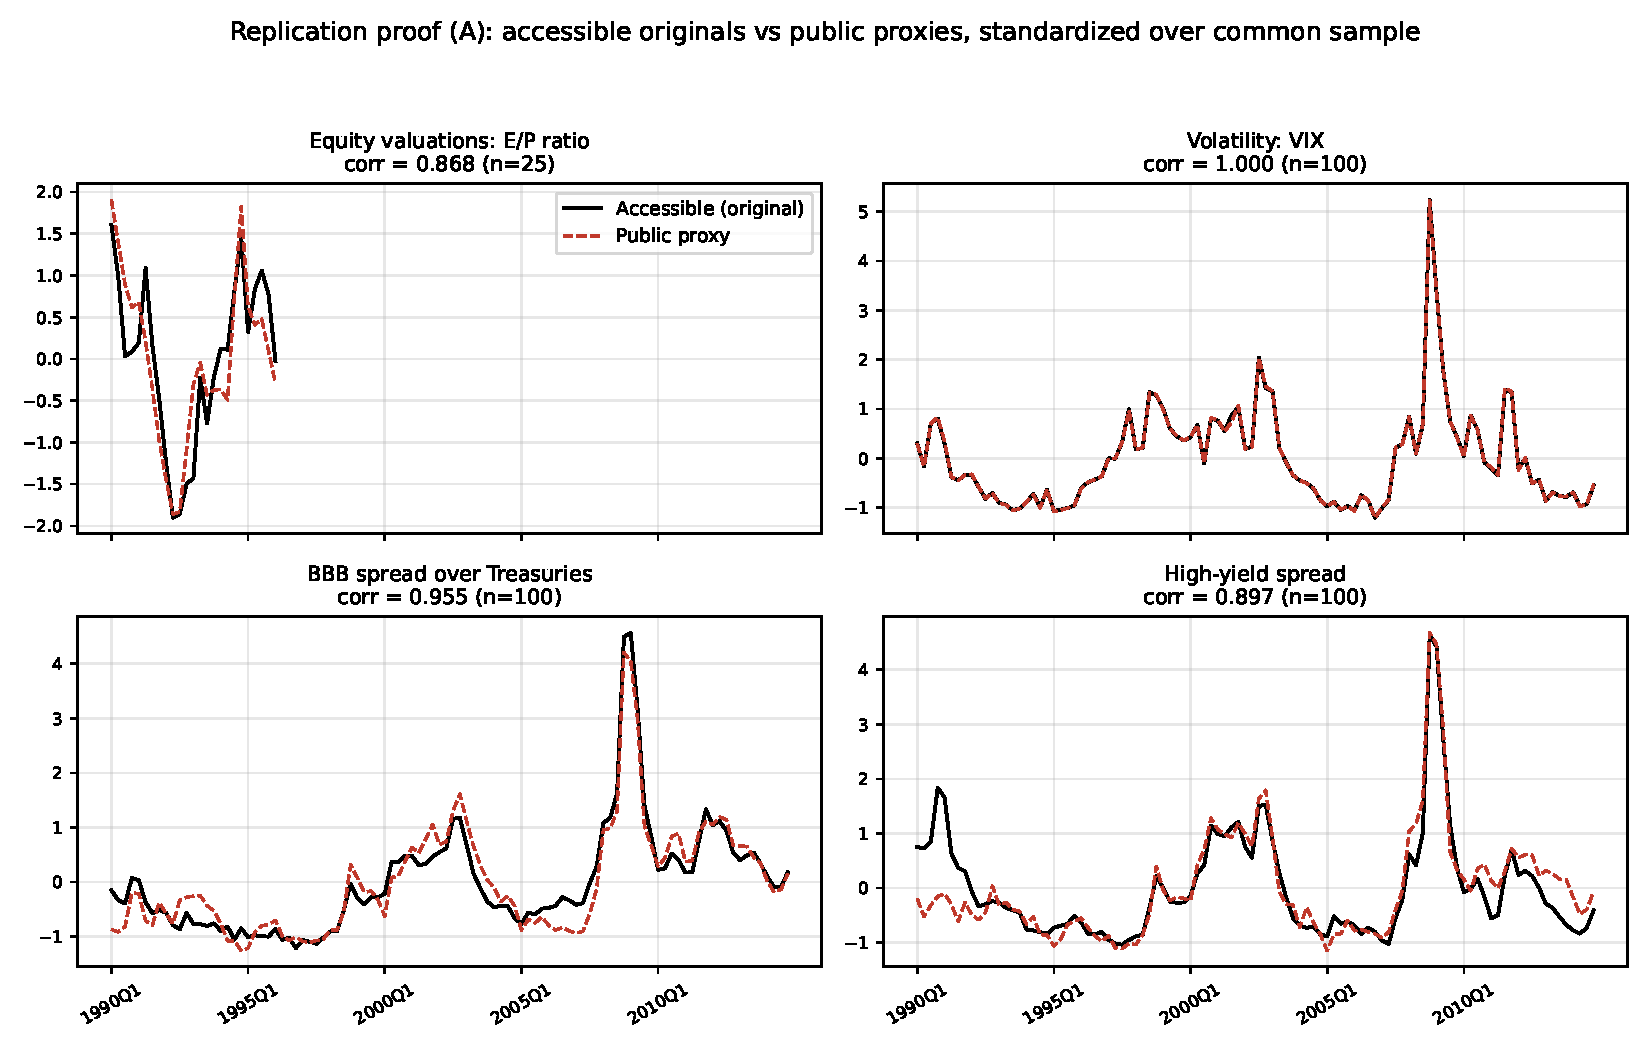
\includegraphics[width=\textwidth]{figures/fig_overlay_A.pdf}
\caption{Replication proof (A): accessible originals vs.\ public proxies,
valuations and volatility.  Standardized over the common sample;
correlation annotated per panel.}
\label{fig:overlayAB}
\end{figure}

\begin{figure}[h]
\centering
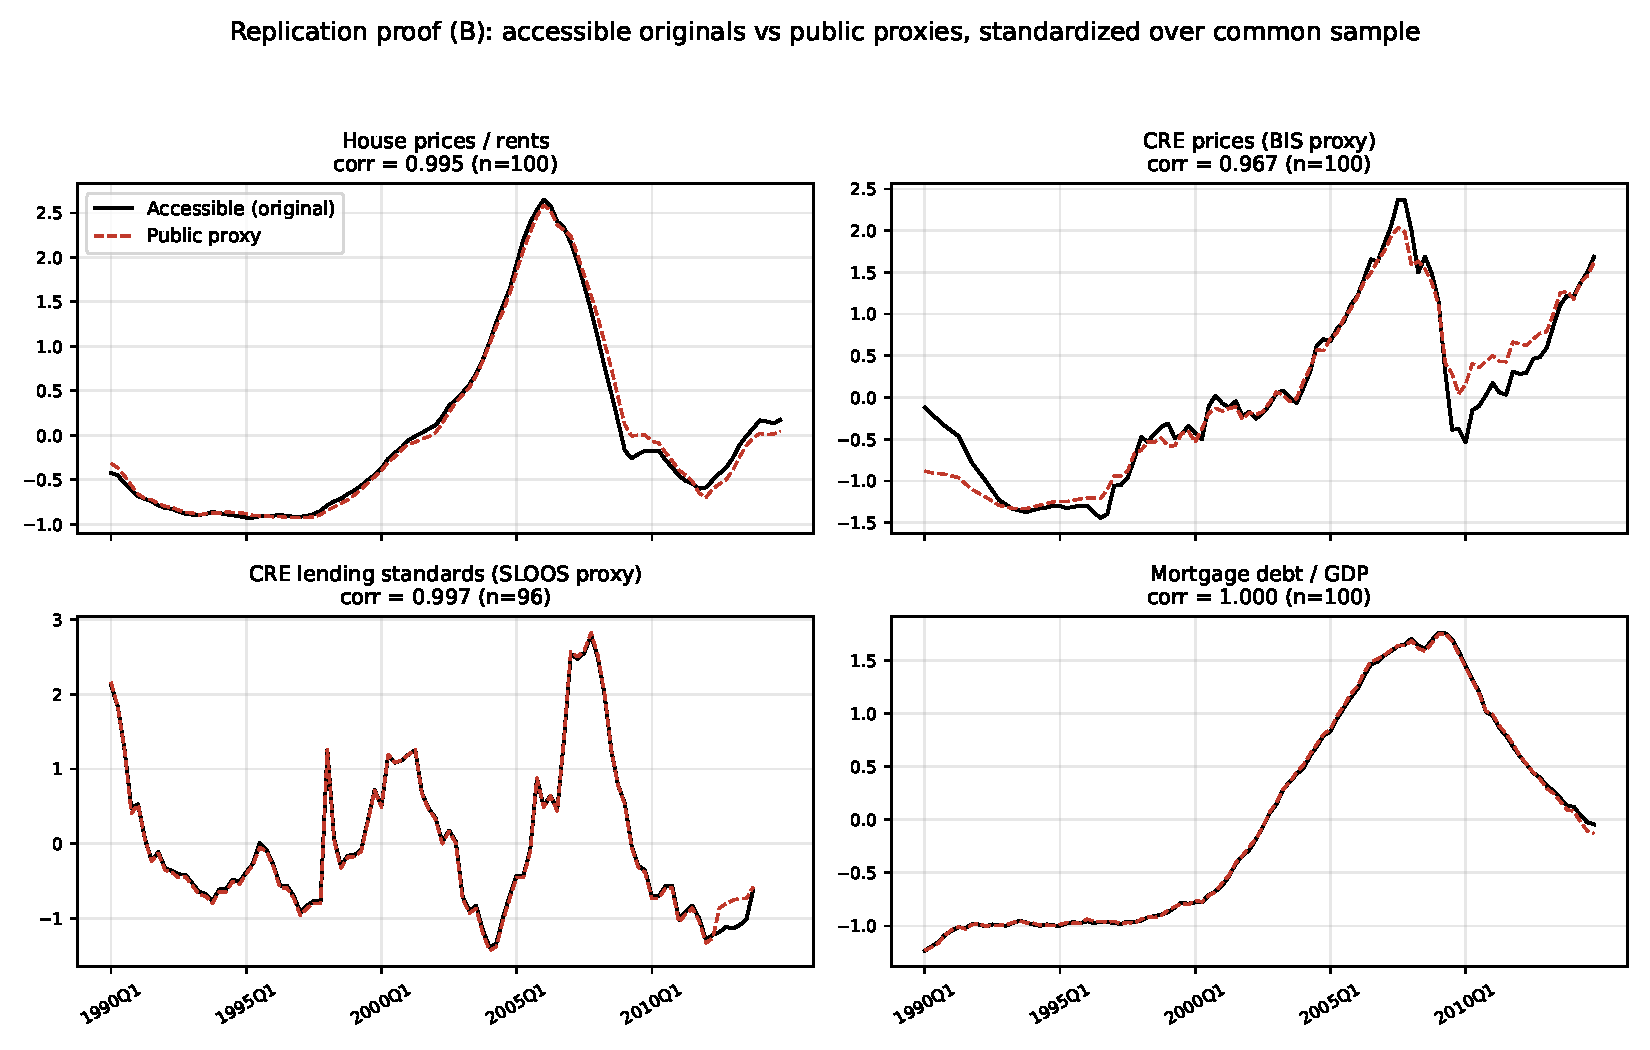
\includegraphics[width=\textwidth]{figures/fig_overlay_B.pdf}
\caption{Replication proof (B): real estate and mortgages.}
\label{fig:overlayBB}
\end{figure}

\begin{figure}[h]
\centering
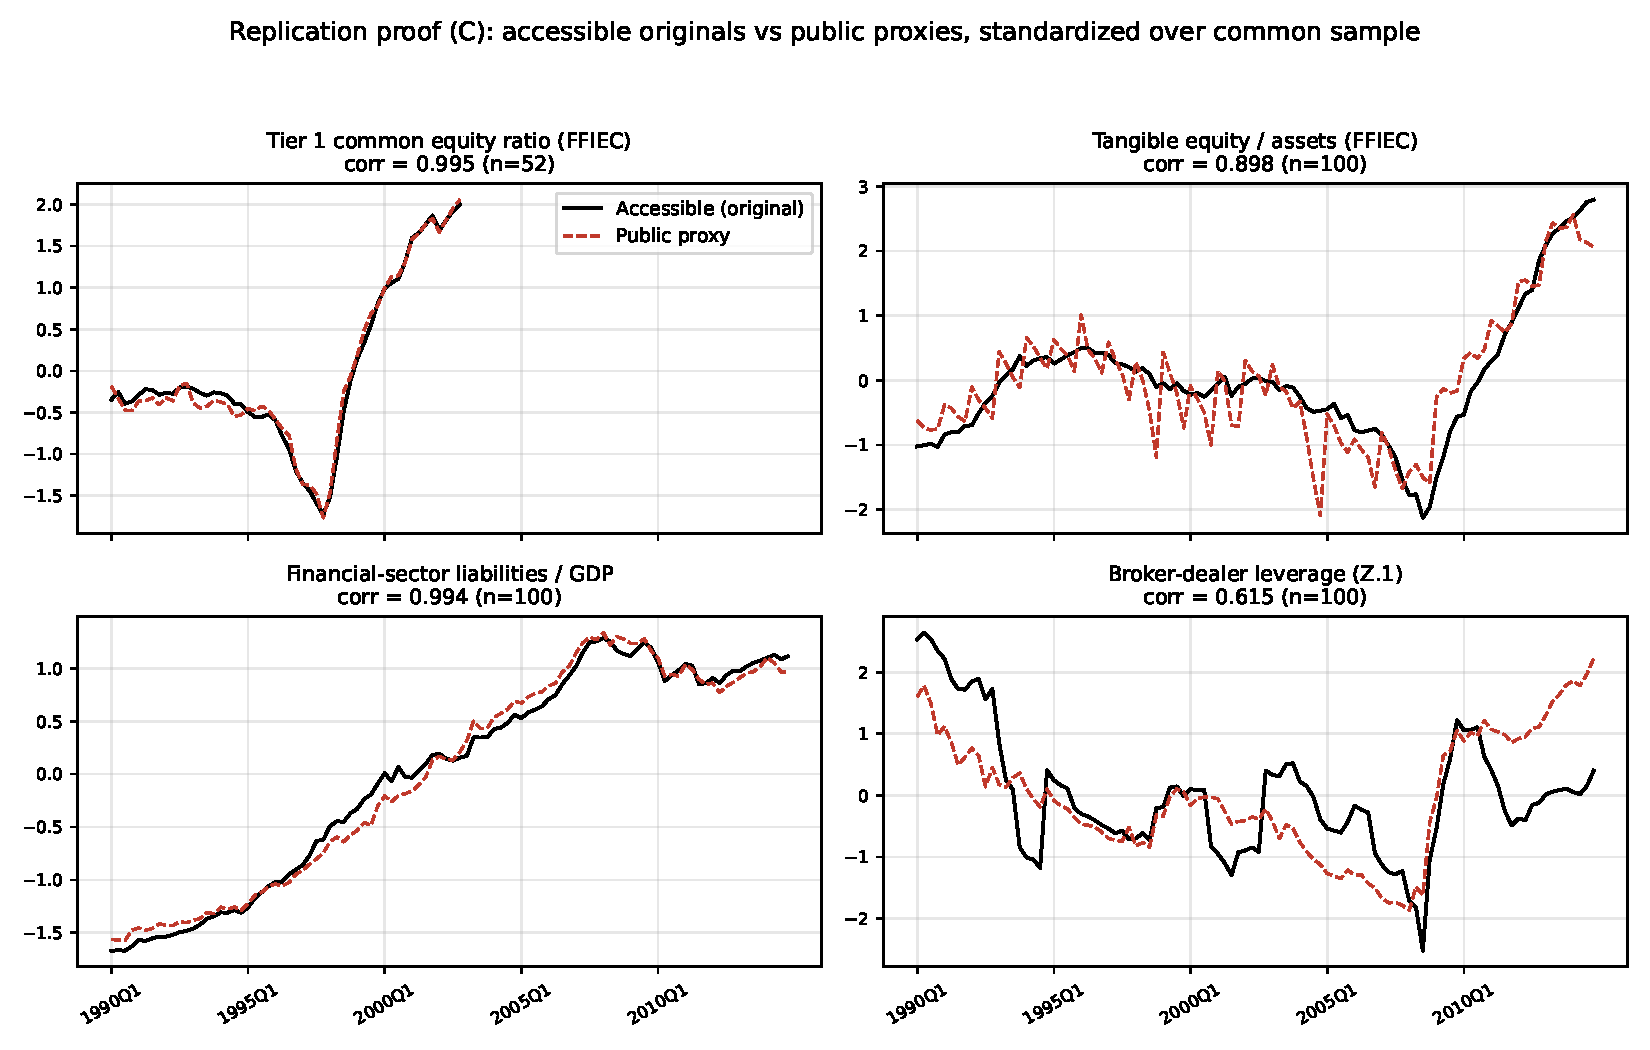
\includegraphics[width=\textwidth]{figures/fig_overlay_C.pdf}
\caption{Replication proof (C): leverage---bank, nonbank, and
financial-sector totals.}
\label{fig:overlayCC}
\end{figure}

\begin{figure}[h]
\centering
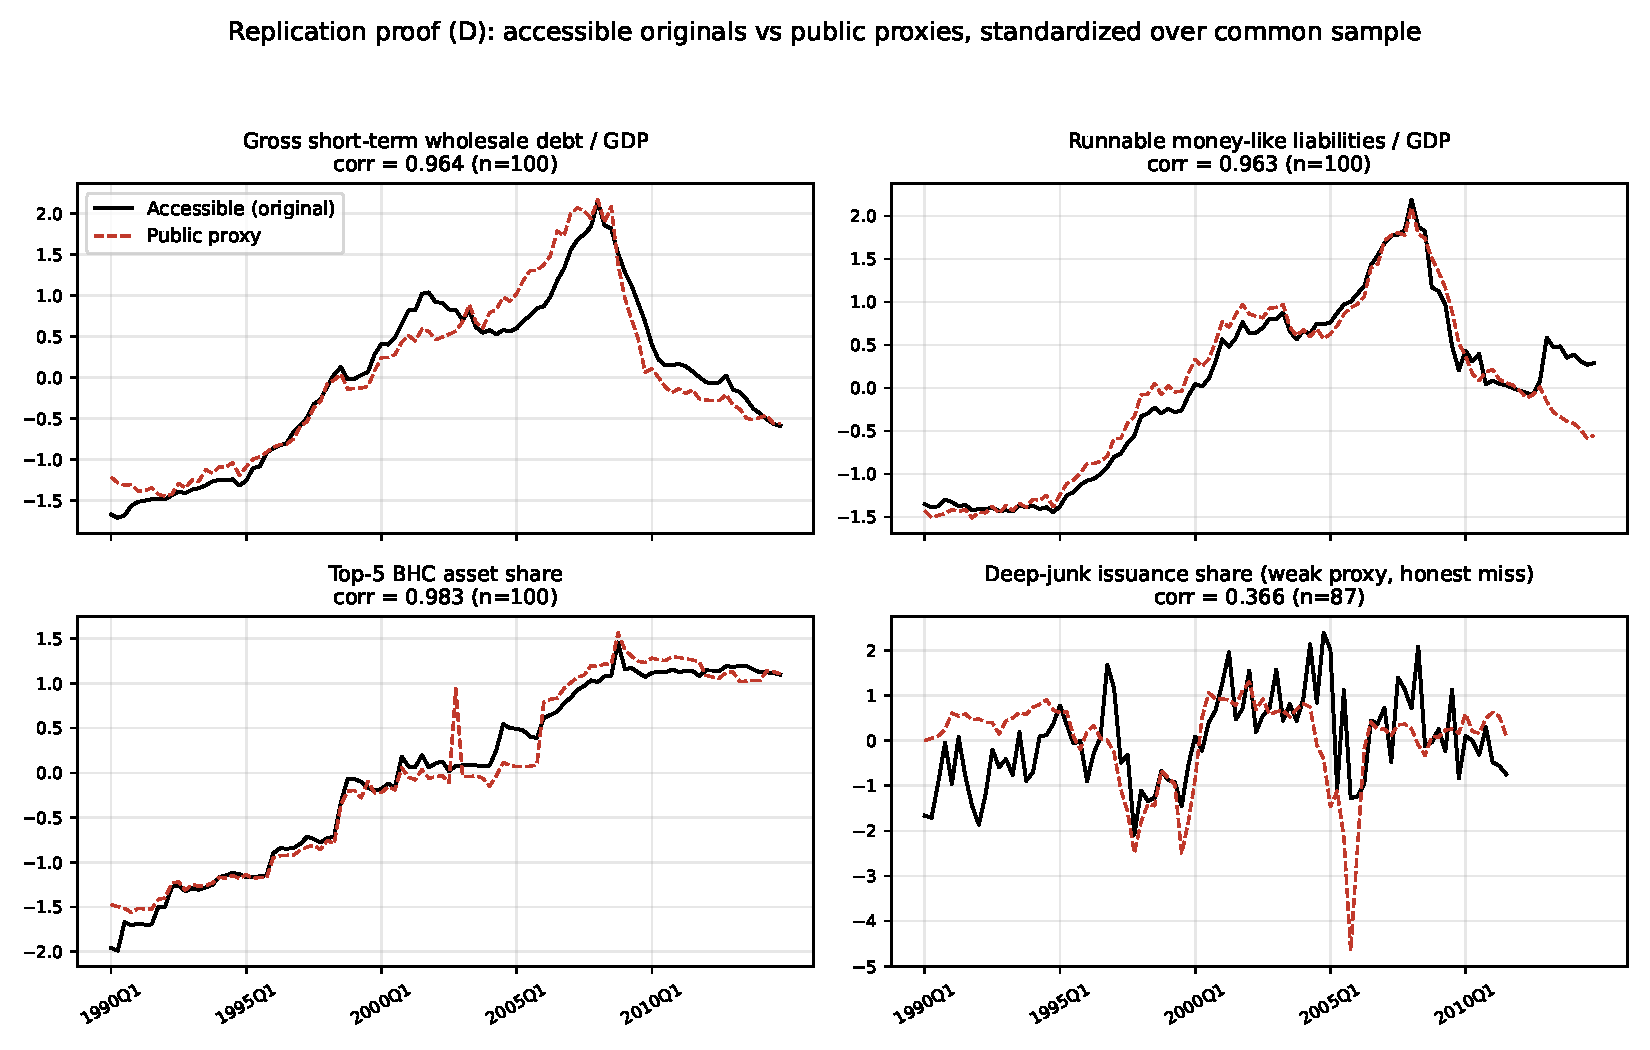
\includegraphics[width=\textwidth]{figures/fig_overlay_D.pdf}
\caption{Replication proof (D): short-term funding, concentration, and
the honest weak proxy (deep-junk issuance share, panel 4).}
\label{fig:overlayCD}
\end{figure}

\subsection{The heat map carried past 2015}

The paper's sample ends 2014Q4, but the public proxies extend further.
The extension runs through 2025Q4 (the last quarter in which all series are
fully observed; 2026Q1 onward is ragged-edge with several series partial or
unpublished).  The two E/P series stop at 2023Q1 (the Yale-hosted Shiller
file has not been updated since September 2023).  The prime-mortgage
SLOOS series ends 2014Q4 (FRED discontinued it); FRED also discontinued
the EQTA bank-leverage aggregate in 2020Q3, where the FFIEC-built tangible
series takes over.  Running the identical pipeline on the unmasked
1990Q1--2025Q4 proxy panel gives the heat map in
Figure~\ref{fig:heatmap}, the aggregate index in
Figure~\ref{fig:aggregate}, and all 14 components in
Figure~\ref{fig:components}.

\begin{figure}[h]
\centering
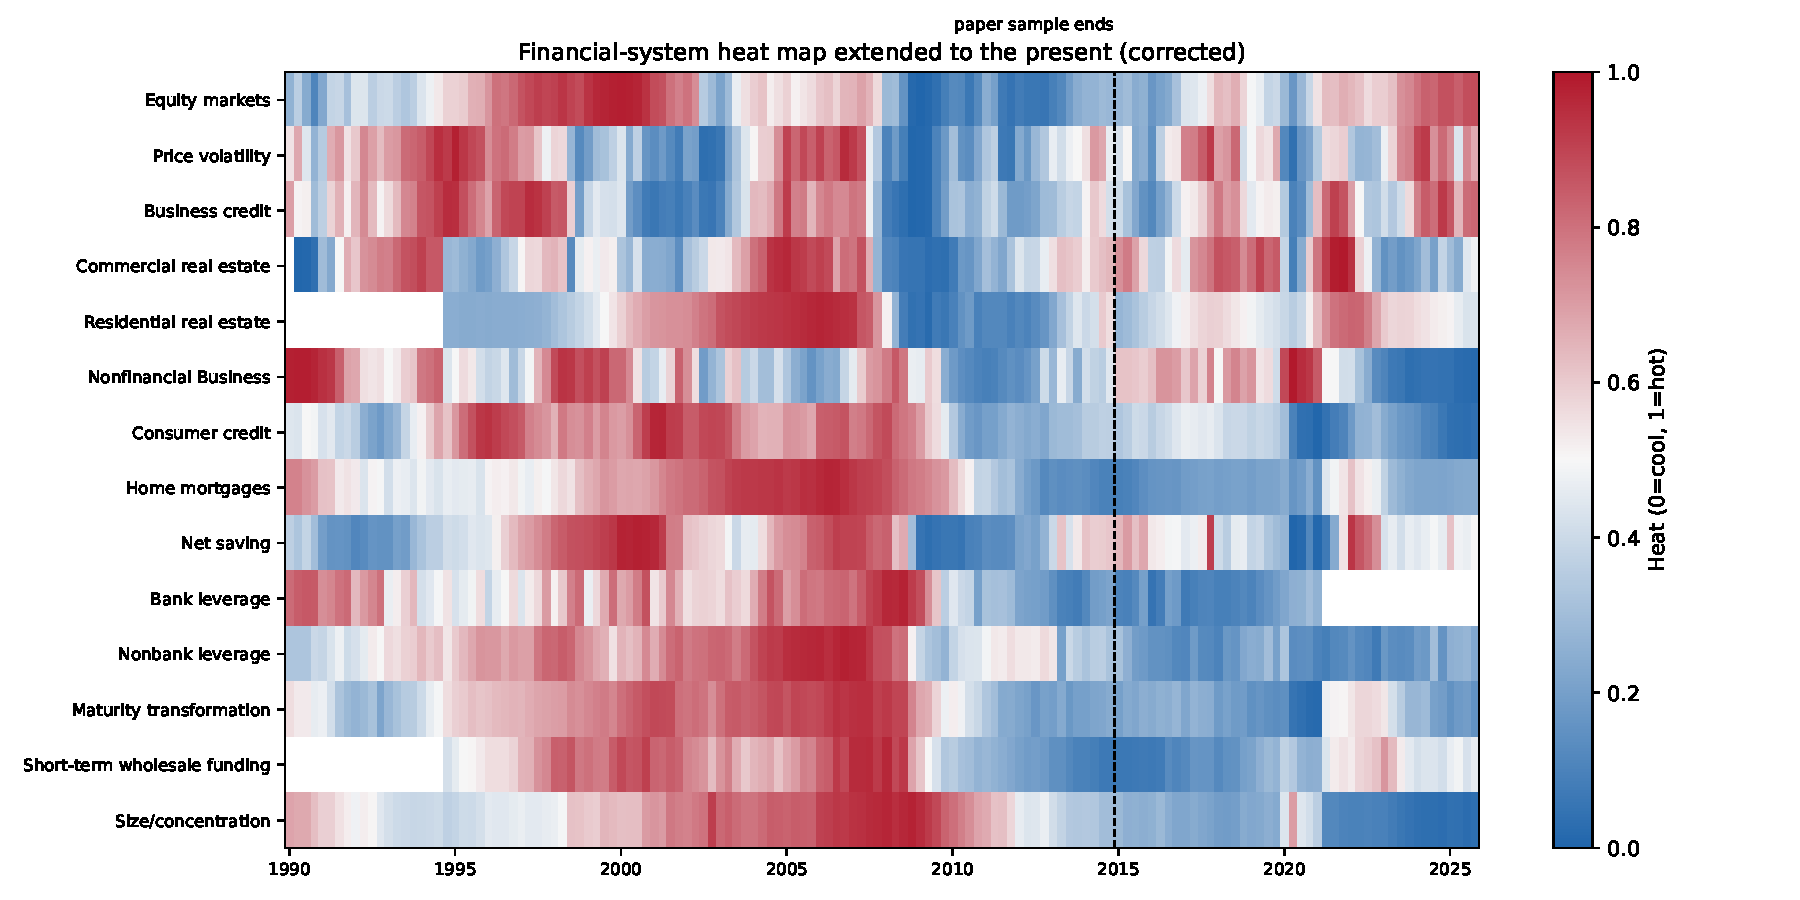
\includegraphics[width=\textwidth]{figures/fig_heatmap_extended.pdf}
\caption{The financial-system heat map extended to the present, from the
43 public proxies.  Blue is cool, red is hot; the dashed line marks the
end of the paper's sample.}
\label{fig:heatmap}
\end{figure}

\begin{figure}[h]
\centering
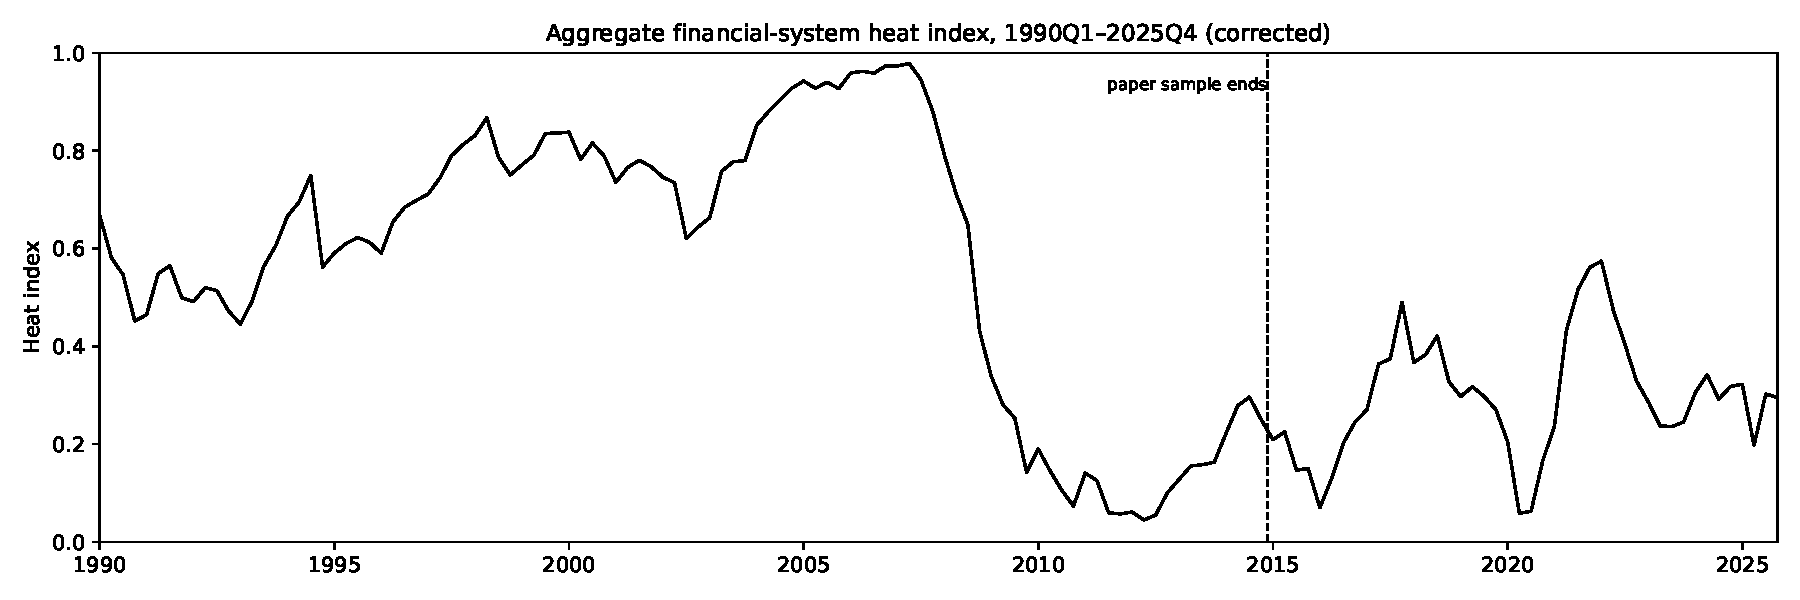
\includegraphics[width=\textwidth]{figures/fig_aggregate_extended.pdf}
\caption{Aggregate financial-system heat index, 1990Q1--2025Q4, from the
public-proxy panel.}
\label{fig:aggregate}
\end{figure}

\begin{figure}[h]
\centering
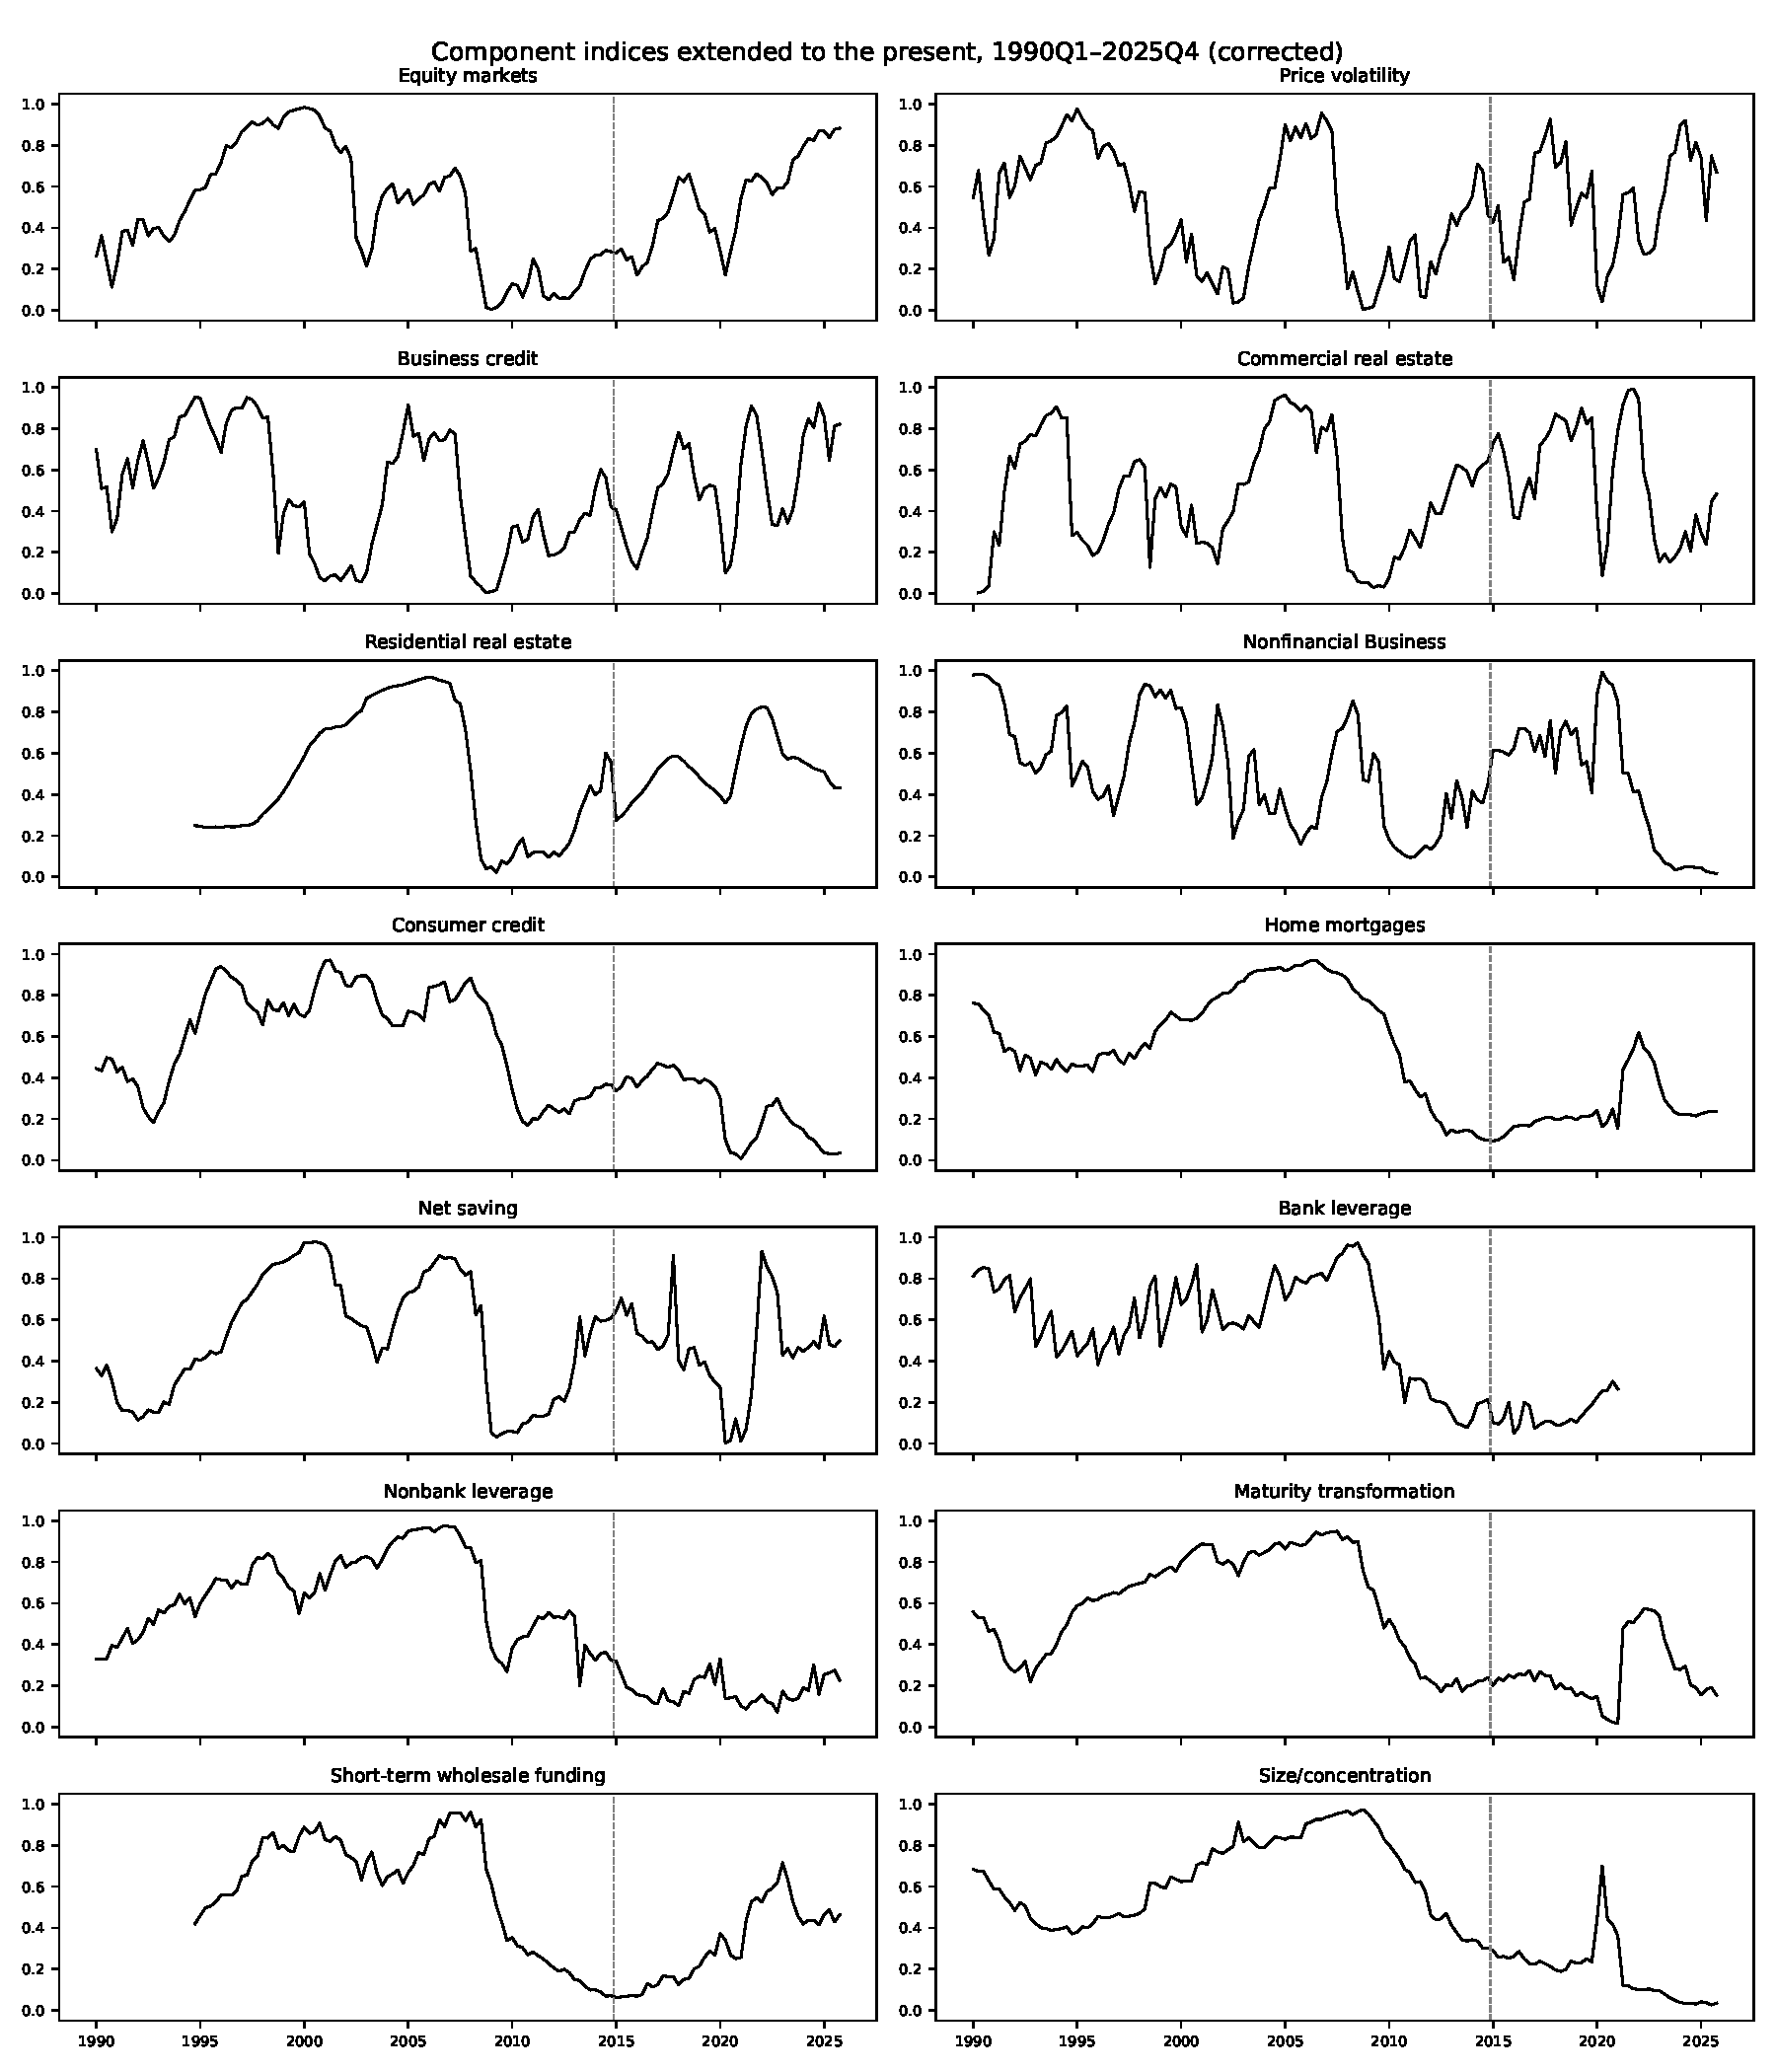
\includegraphics[width=\textwidth]{figures/fig_components_extended.pdf}
\caption{All 14 component indices extended to the present.}
\label{fig:components}
\end{figure}

Three readings, stated plainly.  \textbf{First, the extension validates
the instrument:} the pre-2015 portion reproduces the paper's story---heat
peaks at 0.98 in 2006Q4--2007Q2 and unwinds through the crisis, exactly
the vulnerability-then-realization pattern the paper documents.
\textbf{Second, the COVID shock barely registers} (aggregate 0.19 in
2020Q1, 0.06 in 2020Q2): the heat map measures complacency and
imbalances, not stress, and the pandemic was an exogenous shock with no
prior buildup---note the sign convention (\S\ref{sec:pipeline}), under
which the VIX spike itself reads as \textit{cool}.  \textbf{Third, the
recent picture is cool to lukewarm:} the aggregate sits at 0.20--0.34
through 2024--2025Q4, with warmth concentrated in business credit
(0.65--0.86 over the last year) and price volatility (0.43--0.75);
household, leverage, and funding components are all cool.

\subsection{Caveats specific to the extension}

\begin{itemize}[nosep]
\item \textbf{History moves when the sample grows.}  Standardization,
the 10-year moving-average detrending, and the kernel-CDF bandwidth are
all computed over the full 1990--2025 sample, so the 1990--2014 component
values differ from both the published and the masked runs (aggregate
correlation 0.96, max absolute deviation 0.36; worst component
size/concentration, 0.59).  The extended map is the same methodology on
a longer sample---it is not point-for-point comparable with the
paper's map.
\item \textbf{Ragged-edge discipline.}  An earlier version of the extension
ran to 2026Q2 and showed a sharp end-of-sample spike in the Nonfinancial
Business component (0 to 0.87 in 2026Q1).  An audit rebuilt all five of
that component's indicators from fresh public sources and found no such
move (0.025 to 0.037); the spike was a data-processing error in the
extended build, a 7.6-sigma discrepancy impossible from the smooth
underlying series.  The extension is therefore truncated at 2025Q4, the
last quarter in which every series is fully observed, and every indicator
is tail-validated (|quarterly change| $>$ 3$\sigma$ flagged) before the
pipeline runs.  See the audit note alongside this paper.
\item \textbf{The equity-markets component is missing from 2023Q1,}
when the Shiller source froze; the aggregate from that quarter is a
13-component mean.
\item \textbf{Vintages.}  Everything is current-vintage public data
against the paper's 2015 vintages; revisions explain part of every
deviation.
\item The CRE pipeline discrepancy (\S\ref{sec:misses}) and the missing
maturity gap carry over unchanged.
\end{itemize}

\section{Reproduction recipe}
\label{sec:recipe}

From an empty directory to the reproduced heat map.  No code from any
repository is needed---only the sources named below and the pipeline in
\S\ref{sec:pipeline}.

\begin{enumerate}
\item \textbf{Ground truth.} Download
\url{https://www.federalreserve.gov/econresdata/feds/2015/files/feds2015059.zip}
and parse the two HTML tables: the 44 raw indicator series (quarterly,
1990Q1--2014Q4) and the published aggregate plus 14 component indices on
$(0,1)$.

\item \textbf{Build each series} per \S\ref{sec:catalog}, aligning every
series to calendar quarters (quarterly means for daily/monthly inputs;
year-on-year changes where specified).  FRED series come from
\url{https://fred.stlouisfed.org/graph/fredgraph.csv?id=SERIES_ID};
\textbf{download with \texttt{curl}, not Python \texttt{urllib}}---the
FRED server stalls non-browser user agents and the download will hang.
The EBP/GZ file comes from
\url{https://www.federalreserve.gov/econres/notes/feds-notes/ebp_csv.csv}
(monthly, columns \texttt{date}, \texttt{gz\_spread}, \texttt{ebp},
\texttt{est\_prob}, from 1973M1).  Shiller's E/P from
\url{http://www.econ.yale.edu/~shiller/data/ie_data.xls}.  Y-9C items
from the Federal Reserve Bank of Chicago's bulk BHCF downloads
(\url{https://www.chicagofed.org/banking/financial-institution-reports/bhc-data}); Call
Report items from the FFIEC Central Data Repository bulk downloads
(\url{https://cdr.ffiec.gov/public/PWS/DownloadBulkData.aspx})
(note: bulk files carry MDRM codes with no descriptive labels---identify
items by code); SLOOS historical XML from the Federal Reserve Board's
SLOOS page
(\url{https://www.federalreserve.gov/datadownload/Choose.aspx?rel=sloos});
origination FICO from Fannie Mae's credit supplements
(\url{https://www.fanniemae.com/about-us/investor-relations/quarterly-and-annual-results});
CRE prices from the BIS property price statistics
(\url{https://www.bis.org/statistics/pp.htm}); NIPA items from the BEA
(\url{https://apps.bea.gov/national/Release/TXT/NipaDataQ.txt});
Z.1 mnemonics from the Federal Reserve Financial Accounts
(\url{https://www.federalreserve.gov/releases/z1/}; also on FRED
under \texttt{BOGZ1}-prefixed codes).

\item \textbf{Score each proxy} against the accessible raw series on the
\textit{transformed} signal (sign, transform, standardization per
\S\ref{sec:pipeline}), over the overlap.  Expect the correlations in
\S\ref{sec:catalog}; large deviations mean a construction error.

\item \textbf{Run the pipeline} (\S\ref{sec:pipeline}) on the 43 proxies,
\textbf{masking each proxy to the accessible raw series' coverage}
before transforming---without this, longer proxy histories change
component composition and the comparison is invalid.  Standardize each
series over its full available sample; the \texttt{ma10} transform uses
a 40-quarter rolling mean with minimum 20 observations.  The kernel CDF
uses the Silverman bandwidth on each component series; the aggregate is
the mean of the 14 $(0,1)$ components, kernel-CDF'd again.

\item \textbf{Verify} against Tables~\ref{tab:pipeline}
and~\ref{tab:endtoend}: aggregate 0.97 on the pipeline check, 0.93 on
the full proxy panel; per-component correlations should match to the
decimals quoted.

\item \textbf{Reproduce the figure:} map each component's $(0,1)$ value
to a blue-to-red color scale per quarter; the rebuilt figure should
match the paper's.
\end{enumerate}

\textbf{Gotchas collected along the way:} FRED stalls non-browser user
agents (use \texttt{curl}'s default UA); the FFIEC bulk files have no
descriptive labels (MDRM codes only); mask proxies to accessible coverage
before the pipeline; the \texttt{ma10} transform drops the first up to
19 quarters; Basel~III breaks Y-9C HC-R comparability in 2014Q1 (use the
pre-2014 mnemonics and stop at 2013Q4); the SLOOS CRE aggregate must be
re-dated back one quarter to match the paper's reference-quarter
convention; current public vintages are revised data while the paper used
2015 vintages---expect small deviations everywhere from revision alone.

\section{Limitations}

\begin{itemize}[nosep]
\item \textbf{Data vintages.} Everything above compares current-vintage
public data against the paper's 2015-vintage tables.  Revisions explain
part of every deviation; they cannot be removed without a 2015-vintage
archive (e.g.\ ALFRED).
\item \textbf{The CRE pipeline discrepancy} (\S\ref{sec:misses}) means
the CRE component cannot be fully reconciled from the paper's
documentation---a finding about the paper, not the proxies.
\item \textbf{The maturity gap} has no public substitute; any live
monitoring implementation needs licensed Call Report microdata or a
redefined indicator.
\item \textbf{Proxy dynamics $\ne$ proxy levels.} Several proxies match
shape but not level (loans/deposits runs $\approx$18--20pp low;
short-term money share $\approx$15\% vs.\ $\approx$21--38\%).  This is by
design: the pipeline standardizes, so only dynamics matter---but anyone
reusing a proxy \textit{outside} this pipeline must not mistake it for
the level.
\item \textbf{Coverage ends 2014Q4} by construction (the paper's sample).
The public proxies extend further, but scoring stops where ground truth
stops.
\end{itemize}

\end{document}
